\section{Publish/Subscribe}
\label{publishsubscribe}
Heutige Internet-Anwendungen weisen einen zunehmend dynamischen und gleichzeitig eigenst�ndigen Charakter auf (siehe \cite{Patrick:ManyFacesPubSub}):
mehr und mehr unabh�ngige und �ber das gesamte Internet verteilte Einheiten bieten Informationen und Dienste an. Ort und Erreichbarkeit dieser Einheiten k�nnen
im Laufe der Zeit stark variieren (siehe auch Abschnitt \ref{Abschnitt:peer_to_peer}).
Diese Eigenschaften lassen das Bed�rfnis nach flexibleren Kommunikationsmodellen aufkommen, die die Forderung nach statischen Verbindungen und st�ndiger
Erreichbarkeit der Dienstapplikationen abschw�chen. Um Applikationsdesigner von der Last dieser Forderungen zu befreien,
sollten spezielle
Middleware-Infrastrukturen herangezogen werden, die eine Vermittlerrolle zwischen den beteiligten Einheiten einnehmen und auf angemessenen Kommunikationsmodellen
basieren. P2P-Systeme tragen der Forderung Rechnung, Ressourcen mehr und mehr zu dezentralisieren und �ber das Internet zu verteilen. Sie bieten dar�ber hinaus ein
besseres Routing innerhalb des Systems (siehe Abschnitt \ref{Abschnitt:peer_to_peer}). Die Frage nach der Art der Kommunikation zwischen den einzelnen Peers bleibt
damit aber unangetastet. Ein Kommunikationsmodell, welches den oben genannten Bed�rfnissen nachkommt, ist Publish/Subscribe (kurz Pub/Sub).

\paragraph{Publish/Subscribe:}
\begin{picturenothere}{1}{5}{\mbox{Publish/Subscribe}}{Abb:Publish_Subscribe}
 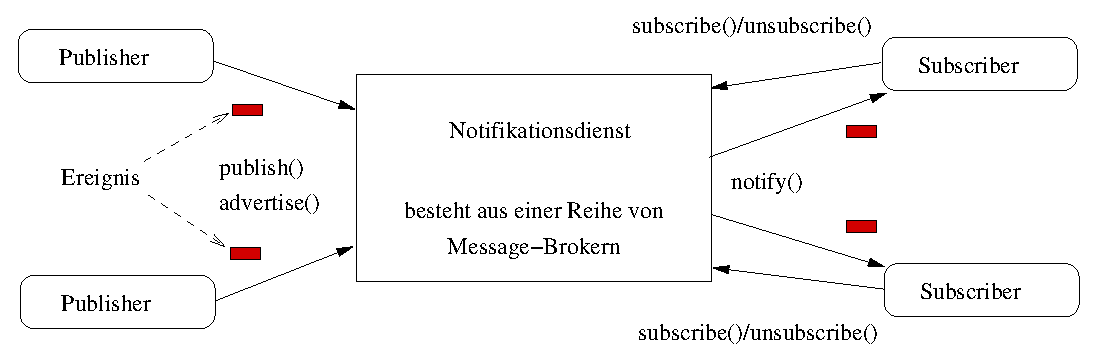
\includegraphics[bb=170 0 544 504 ,scale=0.7]{PubSub}
\end{picturenothere}

Das Pub/Sub-Kommunikationsmodell sieht zun�chst zwei Einheiten vor: Publisher, welche Ereignisse im weitesten Sinne publizieren und Subscriber, welche ihr Interesse
an speziellen Ereignissen oder einer Gruppe von Ereignissen durch Abonnements bzw. Subskriptionen bekunden k�nnen. Subscriber k�nnen �ber das Auftreten von
Ereignissen, die dem bekundeten Interesse entsprechen, durch Notifikationen unterrichtet werden. Hier favorisiert man eine asynchrone Methode der Benachrichtigung
aller Subscriber. Die St�rke dieses ereignisbasierten Interaktionsschemas liegt in der Entkopplung von {\itshape Zeit}, {\itshape Raum} und
{\itshape Synchronisation} zwischen Publisher
und Susbcriber (siehe \cite{Patrick:ManyFacesPubSub}). Im Basis-Interaktionsmodell von Pub/Sub geht von man von einem Notifikationsdienst aus, der Notifikationen
entgegennehmen, zwischenspeichern und weiterleiten kann (siehe Abbildung \ref{Abb:Publish_Subscribe}). Ein Notifikationsdienst besteht in der Regel aus einer Reihe 
von Message-Brokern, die untereinander in einer netzartigen Struktur verbunden sind.\\

Um sein Interesse zu bekunden, ruft ein Subscriber �blicherweise eine Operation \texttt{sub\-scribe()} des Notifikationsdienstes auf. H�ufig kann dabei eine
Reihe von Filterregeln definiert werden, die die Menge der Ereignisse eingrenzen bzw. erweitern, f�r die sich der Subscriber interessiert (zu Filtern siehe
\cite{MuFiBu:2002:FilterSimilarities,Muehl:2001:GenericConstraints}). Diese Informationen
bleiben auch bei Abwesenheit des Subscribers im Notifikationssystem gespeichert und werden erst durch Aufruf der Operation \texttt{un\-sub\-scribe()} gel�scht.\\

Ein Publisher stellt durch Aufruf der Operation \texttt{publish()} dem Notifikationsdienst neue Ereignisse zur Verf�gung. Mit der Operation \texttt{ad\-ver\-tise()}
kann ein Publisher zuk�nftige Ereignisse ank�ndigen. Der Notifikationsdienst kann mit der Operation \texttt{notify()} alle Subscriber �ber die Ereignisse
unterrichten, die auf die angegebenen Filterregeln passen.\\

Die Entkopplung zwischen Publisher und Subscriber erfolgt in drei Dimensionen \cite{Patrick:ManyFacesPubSub}:
\begin{description}
\item [- Raum:] Die beteiligten Parteien Publisher und Subscriber brauchen sich gegenseitig nicht zu kennen. Die Verbindung erfolgt �ber das Notifikationssystem.
  Das hat den Vorteil, dass Publisher nicht eine m�glicherweise gro�e Anzahl von Subscribern verwalten m�ssen. Im Gegenzug k�nnen sich Subscriber auf die Definition
  ihrer Interessen beschr�nken und k�nnen von Lokalit�t und Verf�gbarkeit der Publisher abstrahieren.
\item [- Zeit:] Es ist nicht erforderlich, dass Publisher und Subscriber zeitgleich interagieren. Ver�ffentlichung von Ereignissen und Benachrichtigung �ber
  Ereignisse k�nnen zeitlich versetzt erfolgen.
\item [- Synchronisation:] Publisher werden beim Erzeugen neuer Ereignisse nicht blockiert. Subscriber k�nnen w�hrend der Ausf�hrung paralleler Aktivit�ten
  benachrichtigt werden.
\end{description}

Es gibt eine Reihe von Pub/Sub-Systemen, die f�r verschiedene Zwecke eingesetzt werden k�nnen, wie z. B. REBECA \cite{MuFiBu:2001:ArchFrameECommApp}, Gryphon
\cite{Gryphon}, HERMES \cite{Pietzuch:2004:HermesPhd}, JEDI \cite{CugolaEtAl:2001:JEDI} oder SIENA \cite{SIENA}. F�r Informationen zu diesen Systemen verweisen wir
auf die in den Literaturangaben verzeichneten Quellen.

%%% Local Variables: 
%%% mode: latex
%%% TeX-master: "diplomarbeit"
%%% End: 
